%
% This document is free; you can redistribute it and/or modify
% it under the terms of the GNU General Public License as published by
% the Free Software Foundation; either version 2 of the License, or
% (at your option) any later version.
%
% This document is distributed in the hope that it will be useful, but
% WITHOUT ANY WARRANTY; without even the implied warranty of
% MERCHANTABILITY or FITNESS FOR A PARTICULAR PURPOSE.  See the GNU
% General Public License for more details.
%
% You should have received a copy of the GNU General Public License
% along with this document; if not, write to the Free Software
% Foundation, Inc., 51 Franklin Street, Fifth Floor, Boston, MA
% 02110-1301, USA.
%
% Author: Bertoli Marco
%
\chapter{JMVA}
\label{cha:jmva}
\section{Architecture of the tool}
JMVA has been designed to be very flexible. One important feature is
the complete separation between GUI and computation engine obtained
through an XML layer as shown in \autoref{fig:jmva:Architecture}.
This architecture allows reuse of the analytic engine in other
projects by simply providing a suitable XML input file (see
\autoref{sec:jmva:XML} for details).

\begin{figure}[htbp]
    \begin{center}
        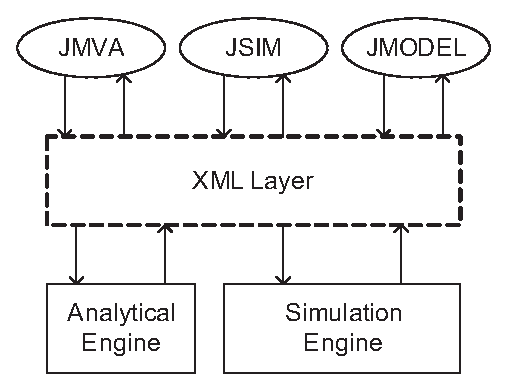
\includegraphics[scale=.65]{img/jmva/Architecture}
    \end{center}
    \caption{JMT Architecture}
    \label{fig:jmva:Architecture}
\end{figure}

Model solution with analytical engine can be started by executing
the \textbf{solve(File XMLFile)} method of the
\textbf{jmt.gui.exact.link.SolverDispatcher} class. The
\texttt{XMLFile} parameter is a well formed XML File according to
\emph{JMTmodel.xsd} schema described in \autoref{sec:jmva:XML}. At
the end of the computation, performance indices will be placed into
the \textbf{solutions} element of input file.

\section{XML format}
\label{sec:jmva:XML}
% Highlight java code
\lstset{language=XML,usekeywordsintag=true, basicstyle=\small} JMVA
XML format is simple and can be written even by hands. The syntax of
that file is specified in \emph{JMTModel.xsd} and is graphically
represented in \autoref{fig:jmva:stylesheet}.

\begin{figure}[p]
    \begin{center}
        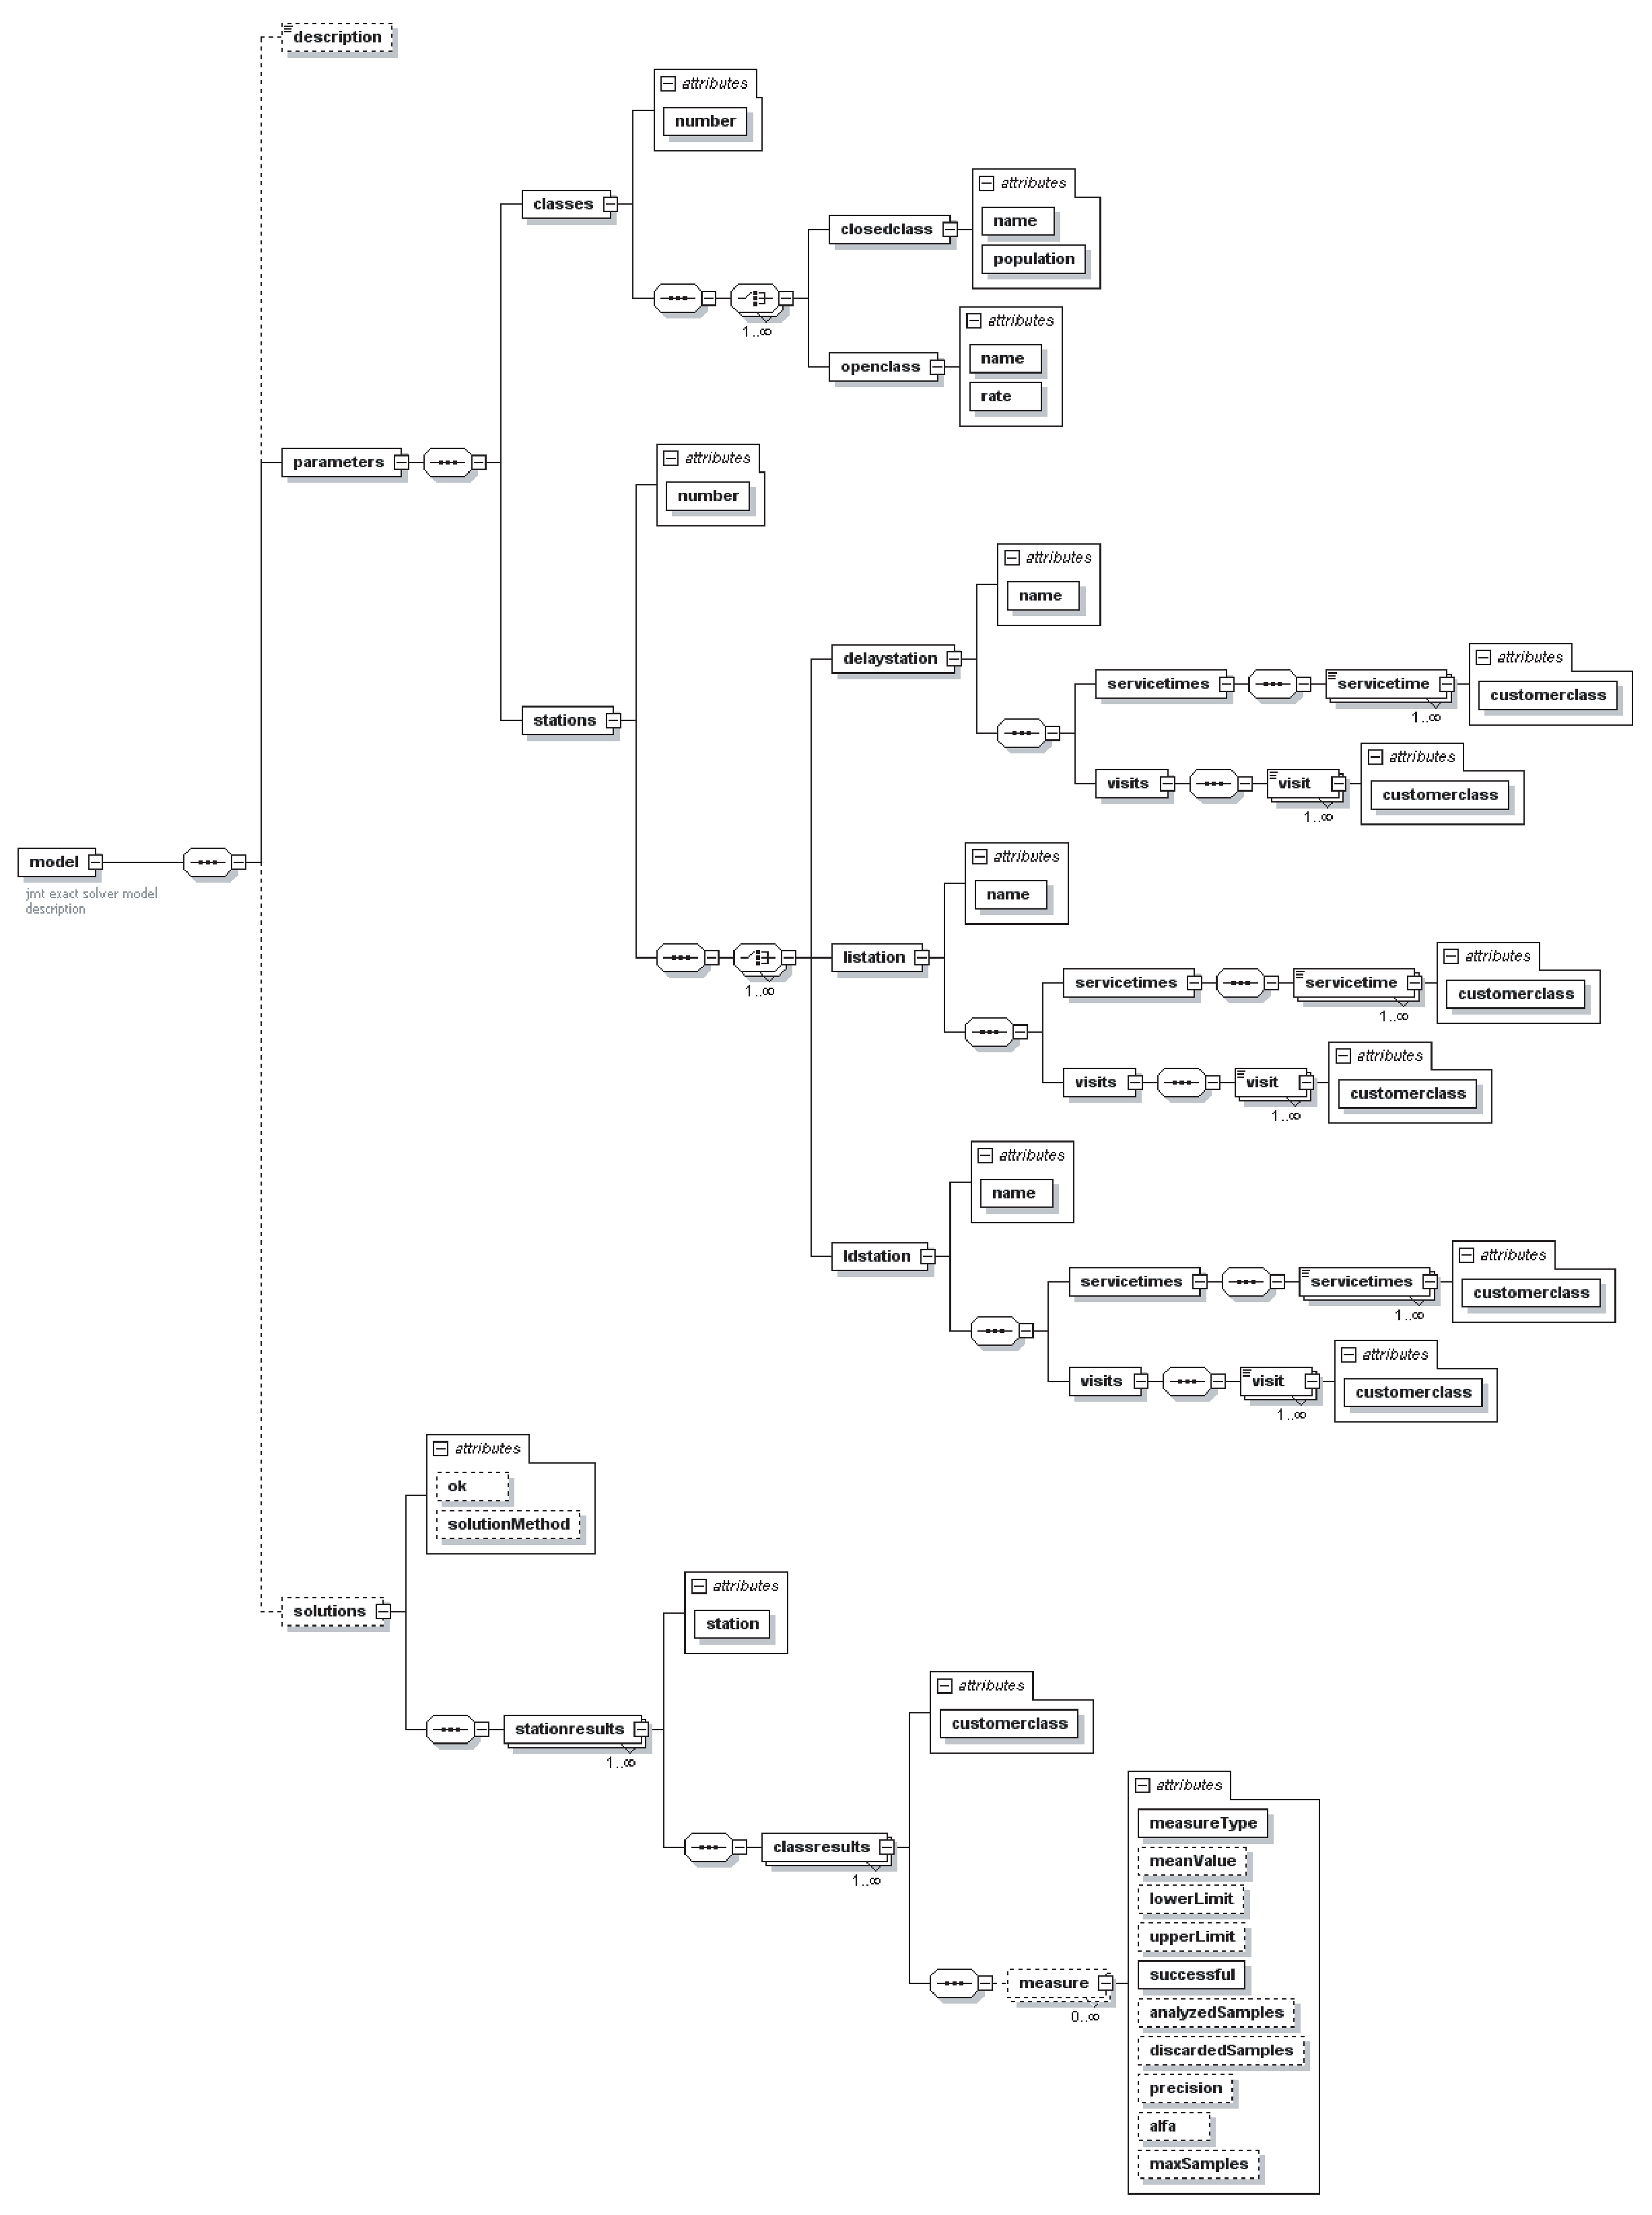
\includegraphics[width=1\textwidth]{img/jmva/JMTmodel}
    \end{center}
    \caption{JMTModel.xsd stylesheet graphic representation}
    \label{fig:jmva:stylesheet}
\end{figure}

The root element is \textbf{model} and can include an optional
\textbf{description} of the model, a section with \textbf{solutions}
(that is parameterized by the solver engine) and the section
\textbf{parameters} used to specify the network to be solved.

The section \textbf{parameters} contains the section
\textbf{classes} that has for attribute the global \textbf{number}
of classes and can include from one to infinite \textbf{openclass}
or \textbf{closedclass}. \textbf{openclass} must specify a
\textbf{name} and arrival \textbf{rate}, while \textbf{closedclass}
must specify a \textbf{name} and \textbf{population}.

For example to define one closed class with $N = 10$ and one open
class with $\lambda = 0.5$ the code will be:

\begin{lstlisting}[gobble=7]
        <classes number="2">
            <closedclass name="ClosedClass" population="10"/>
            <openclass name="OpenClass" rate="0.5"/>
        </classes>
\end{lstlisting}

The other section of \textbf{parameters} is \textbf{stations}. This
element has \textbf{number} as attribute (like classes) and is
composed from one to infinite elements of the following types:
\begin{description*}
    \item[delaystation] is a delay station (infinite server)
    \item[listation] is a load independent station
    \item[ldstation] is a load dependent station
\end{description*}
All the elements are defined with the same procedure. For each
station the \textbf{name} attribute should be specified and two
elements named \textbf{servicetimes} and \textbf{visits} must be
included. \textbf{servicetimes} must include a list of at least one
\textbf{servicetime} element and \textbf{visits} must include a list
of at least one \textbf{visit} element. Both \textbf{visit} and
\textbf{servicetime} elements have a \texttt{double} numeric value
and each element has an attribute named \textbf{customerclass} that
is used to associate a value of service time/visit with the
corresponding customer class.

The only exception is \textbf{servicetime} parameter for a load
dependent station. In this case the value is not a double but is a
list of \texttt{double} separated by the special character
\textbf{;} . The list is ordered for ascending values of number of
jobs in the station, starting from 1 to number of customer $N$ of
the closed class of the model.

For example in a model with one closed class, named \emph{Class1},
with $N=5$ and three stations: a load independent with service
demand 1, a delay with service demand 2 and a load dependent with
$D(N)=N+2$, the following code should be used for the station
definition:

\begin{lstlisting}[gobble=7]
        <stations number="3">
            <listation name="LoadIndependent">
                <servicetimes>
                    <servicetime customerclass="Class1">
                        1.0</servicetime>
                </servicetimes>
                <visits>
                    <visit customerclass="Class1">1.0</visit>
                </visits>
            </listation>
            <delaystation name="Delay">
                <servicetimes>
                    <servicetime customerclass="Class1">
                        2.0</servicetime>
                </servicetimes>
                <visits>
                    <visit customerclass="Class1">1.0</visit>
                </visits>
            </delaystation>
            <ldstation name="LoadDependent">
                <servicetimes>
                    <servicetimes customerclass="Class1">
                        3.0;4.0;5.0;6.0;7.0</servicetimes>
                </servicetimes>
                <visits>
                    <visit customerclass="Class1">1.0</visit>
                </visits>
            </ldstation>
        </stations>
\end{lstlisting}

Also the computed performance indices are stored in the same XML
document. \textbf{solutions} has two attributes: \textbf{ok} that
indicates if the computation was successful and
\textbf{solutionMethod} that indicates if solution was obtained
through analytical engine or simulator. Inside a \textbf{solutions}
element there is a list of one or more \textbf{stationresults}, an
element with station \textbf{name} as its attribute that contains
one or more \textbf{classresults}, an element with class name
(\textbf{customerclass}) as its attribute. This peculiar structure
is needed to store a matrix of results. Each \textbf{classresults}
element contains any number of \textbf{measure} elements that are
used to store computed performance indices. \textbf{measure} has the
following attributes:
\begin{description}
\item[measureType] type of performance index, can be one between \emph{Queue
length}, \emph{Throughput}, \emph{Residence time} and
\emph{Utilization}
\item[successful] boolean field that indicates if measure was
computed correctly
\item[meanValue] (optional) computed value. This field is optional
and will be always present if successful=true
\item[lowerLimit] (optional) lower limit of confidence interval. As
MVA produces \emph{exact} solution, this field is used only when
model is solved with simulator
\item[upperLimit] (optional) upper limit of confidence interval. As
MVA produces \emph{exact} solution, this field is used only when
model is solved with simulator
\item[analyzedSamples] (optional) number of samples analyzed by the
simulator
\item[discardedSamples] (optional) number of samples discarded by the
simulator
\item[precision] (optional) maximum relative error allowed by
simulator
\item[alfa] (optional) confidence interval required to simulator
\item[maxSamples] (optional) maximum number of samples allowed by
simulator
\end{description}
Note that only the first three elements of the above description
will be saved by JMVA. The others are used when the model is solved
using the simulator JSIM. For example, a model with one class (named
\emph{Class1}) and two stations (named \emph{Station1} and
\emph{Station2}) will produce the following solutions:
\begin{lstlisting}[gobble=3]
    <solutions ok="true" solutionMethod="analytical">
        <stationresults station="Station1">
            <classresults customerclass="Class1">
                <measure meanValue="9.930828575679609"
                    measureType="Queue length"
                    successful="true"/>
                <measure meanValue="5.467534818643117"
                    measureType="Throughput"
                    successful="true"/>
                <measure meanValue="1.8163265356477696"
                   measureType="Residence time"
                   successful="true"/>
                <measure meanValue="0.9999999999987986"
                    measureType="Utilization"
                    successful="true"/>
            </classresults>
        </stationresults>
        <stationresults station="Station2">
            <classresults customerclass="Class1">
                <measure meanValue="0.06917142432039082"
                    measureType="Queue length"
                    successful="true"/>
                <measure meanValue="5.467534818643117"
                    measureType="Throughput"
                    successful="true"/>
                <measure meanValue="0.01265130019557098"
                    measureType="Residence time"
                    successful="true"/>
                <measure meanValue="0.06469628980696993"
                    measureType="Utilization"
                    successful="true"/>
            </classresults>
        </stationresults>
    </solutions>
\end{lstlisting}

It is important to point out that JMVA stores and loads model and
results in \emph{exactly} the same XML format used to dialogue with
the analytical engine. The best practice to learn rapidly its syntax
is to create a model using JMVA GUI, store it in any place and open
it with a text editor.
